\documentclass{article}
\usepackage[utf8]{inputenc}
\usepackage[T1]{fontenc}
\usepackage{graphicx}
\usepackage{hyperref}
\begin{document}
\begin{titlepage}
\begin{center}
    
\includegraphics[height = 125pt]{FIT_barevne_CMYK_CZ.pdf} \\
    \begin{LARGE}
    	\textsc{\textbf{IFJ PROJECT DOCUMENTATION}}
    	\\[10mm]
    	\textsc{\textbf{2022}}
    \end{LARGE}
    \\[50mm]
    \begin{LARGE}
        \textsc{\textbf{TEAM XVECER29, BST VARIANT}}
    \end{LARGE}
    \\[25mm]
\begin{table}[h]
\centering
\begin{large}
    \begin{tabular}{l l l l}
         Petr Večeřa & xvecer29 & 25\% & leader\\[2mm]
         Matěj Šmida & xsmida06 & 25\% &\\[2mm]
         René Češka & xceska06 & 25\% &\\[2mm]
         Josef Unčovský & xuncov00 & 25\% &
    \end{tabular}
\end{large}
\end{table}
\end{center}
\end{titlepage}
\tableofcontents
\newpage
\section{Introduction}
This document was created as documentation for the IFJ project, describing implementation methods of all compiler components as well as problems during said implementation.
\section{Compiler components}
The task was to create a compiler of the \textbf{IFJ22} language, which is based on PHP 8, into the \textbf{IFJcode22} language. Since our team has chosen the BST variant of the task, table of symbols had to be implemented as a binary search tree.
The compiler consists of the following components:
\begin{itemize}
    \item Lexical analyzer
    \item Syntactic analyzer
    \item Semantic analyzer
    \item Code generator
\end{itemize}
The input code is processed by each component in the same order as written in the list above.
\subsection{Lexical analyzer}
The task of the lexical analyzer is to load individual lexical units (lexemes) and transform them into tokens, which represent the lexemes further on in other components of the compiler. The lexical analyzer component is implemented in the \textbf{scanner.c} module using a \textbf{finite state machine}. For situations in which an unrecognizable input token is provided, we use the \textbf{NOT\_TOKEN} label. The parser component then contains a check for \textbf{NOT\_TOKEN}, terminating the program upon encounter.
\newline
\begin{figure}
\begin{center}
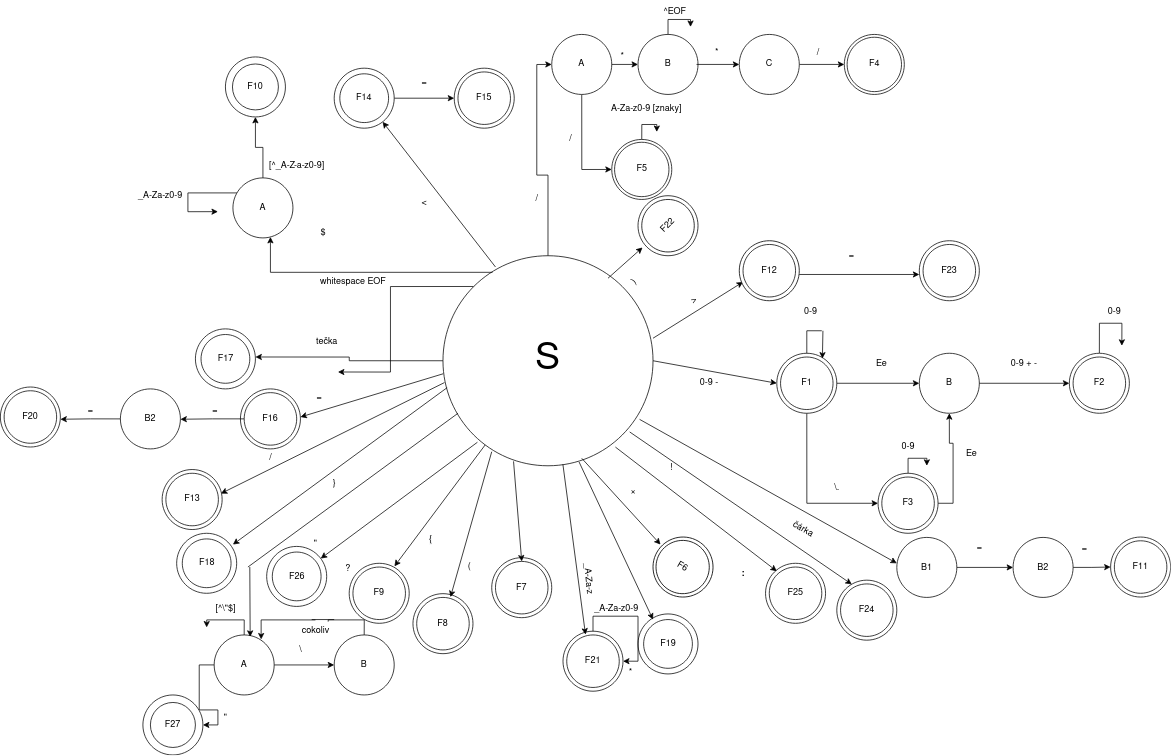
\includegraphics[height = 300pt]{fsm.png}
\caption{Finite state machine}
\label{fig:1}
\end{center}
\end{figure}
\newpage
\subsection{Syntactic analyzer}
The task of the syntactic analyzer is to fill the table of symbols (symtable). The component is implemented in the \textbf{parser.c} module and its input is a token from lexical analyzer. We used the top-down approach for implementation, precisely using \textbf{recursive descent}, which is based on LL grammar and LL table. 
\subsubsection{LL grammar}
\begin{enumerate}
    \item <PROLOG> $\rightarrow$ <?php declare(strict\_types=1);  <PROGRAM>
    \item <PROGRAM> $\rightarrow$ <PROG\_BODY>  ?> EOF
    \item <FUNC> $\rightarrow$ function ID (<PARAMS>) : <RETURN\_EXPRESSION> \{<BODY>\}
    \item <FUNC\_CALL> $\rightarrow$ ID(<CALL\_PARAMS>);
    \item <CALL\_PARAMS> $\rightarrow$ $\epsilon$
    \item <CALL\_PARAMS> $\rightarrow$ \$ID <CALL\_PARAMS\_N>
    \item <CALL\_PARAMS\_N> $\rightarrow$ $\epsilon$
    \item <CALL\_PARAMS\_N> $\rightarrow$ ,\$ID <CALL\_PARAMS\_N>
    \item <PARAMS> $\rightarrow$ $\epsilon$
    \item <PARAMS> $\rightarrow$ \$ID <PARAMS\_N>
    \item <PARAMS\_N> $\rightarrow$ $\epsilon$
    \item <PARAMS\_N> $\rightarrow$ , \$ID <PARAMS\_N>
    \item <PROG\_BODY> $\rightarrow$ <FUNC> <PROG\_BODY>
    \item <PROG\_BODY> $\rightarrow$ $\epsilon$
    \item <PROG\_BODY> $\rightarrow$ <EXPRESSION>; <PROG\_BODY>
    \item <PROG\_BODY> $\rightarrow$ ; <PROG\_BODY>
    \item <PROG\_BODY> $\rightarrow$ <CONSTRUCT> <PROG\_BODY>
    \item <ASSIGNMENT> $\rightarrow$ \$ID = <EXPRESSION>;
    \item <ASSIGNMENT> $\rightarrow$ \$ID = <FUNC\_CALL>;
    \item <EXPRESSION> $\rightarrow$ <RETURN>
    \item <CONSTRUCT> $\rightarrow$ <ASSIGNMENT>
    \item <CONSTRUCT> $\rightarrow$ <WHILE\_LOOP> <CONSTRUCT>
    \item <CONSTRUCT> $\rightarrow$ if (<EXPRESSION>) \{<BODY>\} else \{<BODY>\}
    \item <CONSTRUCT> $\rightarrow$ while (<CONSTRUCT>) \{<BODY>\}
    \item <RETURN> $\rightarrow$ return <RETURN\_EXPRESSION>;
    \item <RETURN\_EXPRESSION> $\rightarrow$ $\epsilon$
    \item <RETURN\_EXPRESSION> $\rightarrow$ <EXPRESSION>
    \item <BODY> $\rightarrow$ $\epsilon$
    \item <BODY> $\rightarrow$ <EXPRESSION>; <BODY>
    \item <BODY> $\rightarrow$ <CONSTRUCT> <BODY>
    \item <BODY> $\rightarrow$ ; <BODY>
\end{enumerate}
\newpage
\begin{table}
\begin{center}
\subsubsection{LL table}

\begin{tabular}{ |c|c|c|c|c|c|c|c|c|c|c|c|c|c|c|c|c| }
\hline
&; & \rotatebox{90}{ID} & \rotatebox{90}{FUNCTION} & : & \rotatebox{90}{\$ID} & \rotatebox{90}{EOF} & , & \rotatebox{90}{IF} & \rotatebox{90}{ELSE} & \rotatebox{90}{WHILE} & \rotatebox{90}{RETURN} & ( & ) & = \\
\hline
<PROLOG>& 16 & & 15 & & & & & & & & & & & \\
\hline
<PROGRAM>& 16 & & 15 & & & 2& & & & & & & & \\
\hline
<FUNC>& & 4 & 4 & 4& & & & & & & & & & \\
\hline
<FUNC\_CALL>& & 5 & & & & & & & & & & & & \\
\hline
<CALL\_PARAMS>& & & & & 7 &  & 7 & & & & & & &\\
\hline
<CALL\_PARAMS\_N>& & & & & 9 & & 9 & & & & & & &\\
\hline
<PARAMS>& & & & & 11 & & & & & & & & &\\
\hline
<PARAMS\_N>& & & & & 13& & 13 & & & & & & &\\
\hline
<BODY>& & & & & & & & 23 & 27 & 24 & & & &\\
\hline
<ASSIGNMENT>& & & & & 17 & & & & & & & & & 17 \\
\hline
<EXPRESSION>& & & 19 & & & & & 20 & & & & & & \\
\hline
<CONSTRUCT>& & & & & & & & 23 & & & & & & \\
\hline
<PROG\_BODY>& & & & & & &  &24 & & 26 & & & & \\
\hline
<RETURN>& & & & & & & & & & & 26 & 4 & 4 & \\
\hline
<RETURN\_EXPRESSION>& & & & & 28 & & & & & & & & &  \\
\hline
\end{tabular}
\caption{LL Table}
\label{tab:1}
\end{center}
\end{table}
\newpage

\newpage
\subsection{Semantic analyzer}
\subsubsection{Expression parsing}
Our team didn't use precedence table, opting for using a combination of postfix conversions, binary and ternary trees instead to parse expressions. An \textbf{arithmetic search tree} (AST) was created for communication between parser and code generator, to help with work parallelization. AST contains all information needed to generate code. The AST is used for parsing expressions as a binary tree. At other instances it is also used as a ternary tree. Logic for parsing expressions is located in the files \textbf{atree.c} and \textbf{stree.c}.
\subsection{Code generator}
Code generator is implemented in the \textbf{generator.c} module. Its task is to create the final code, in our case \textbf{IFJcode2022} code. Code generator takes the tree structure passed from parser as input, nodes of which contain information about individual commands. The main component is node type \textbf{n\_stList}, which acts as a list of individual commands in individual functions (command in the left node, another \textbf{n\_stList} in the right node). 
Most of the nodes are generated recursively. The final generated code uses stack to pass on information.
Generator also generates helping functions on the first rows of the source file written in IFJCODE, which are used in all individual generated commands.
Since generating variables in loops proved to be complicated, all variable definitions are moved to a label which is then called at the beginning of a function. Functions (and what they return) are processed according to the \textbf{varT table}.
\newpage
\begin{table}
\begin{center}
\subsubsection{varT table}
\begin{tabular}{ |c|c|c|c|c|c|c|c|c|c|c|c|c|c|c| }
\hline
\rotatebox{90}{node type} & \rotatebox{90}{left node} & \rotatebox{90}{middle node} & \rotatebox{90}{right node} & \rotatebox{90}{cmpT} & \rotatebox{90}{varT} & \rotatebox{90}{name} & \rotatebox{90}{valueInt} & \rotatebox{90}{valueFloat} & \rotatebox{90}{valueString} & \rotatebox{90}{isNullable}\\
\hline
n\_stList& any & & n\_stList/null & & & & & & & \\
\hline
n\_mul& any & & any & & & & & & & \\
\hline
n\_add& any & & any & & & & & & &\\
\hline
n\_sub& any& & any& & & & & & &\\
\hline
n\_div&any & &any & &  &  & & & &\\
\hline
n\_concat&any & & any & & & && & &\\
\hline
n\_comp& any& &any & set & & & & & &\\
\hline
n\_constant& & & & &set & & set&set & set &\\
\hline
n\_var& & & & & &set & & & &\\
\hline
n\_assignVar& & &any & & &set & & & &\\
\hline
n\_defvar& & &any & & & set& &  & &\\
\hline
n\_write& any & & & & & & &  & &\\
\hline
n\_read& n\_argLcall & & & & & &  & & & \\
\hline
n\_if&n\_comp/n\_var/n\_cons& any &any & & & & & & &\\
\hline
n\_while&n\_comp/n\_var/n\_cons & any & & & & & & & &\\
\hline
n\_funDef&n\_argLfun & & & &set &set & & & &\\
\hline
n\_argLfun& & &n\_argLfun & &set &set & & & &set\\
\hline
n\_funCall&n\_argLcall & & & & & set& & & &\\
\hline
n\_argLcall&any & &n\_argLcall & & & & & & &\\
\hline
n\_return& & & any& & set & & & & &set\\
\hline
\end{tabular}
\caption{varT Table}
\label{tab:2}
\end{center}
\end{table}
\newpage
\section{Division of labour \& Teamwork}
From the release of the project description, weekly meetings were held consistently until the end of the deadline. \textbf{Doodle} has been used for scheduling the meetings. We used \textbf{Git} as a version control system hosted on \textbf{GitLab}. A testing pipeline was created for every file entering the master branch, ensuring less errors overall. Because of the amount of various components, that had to be implemented, \textbf{Trello} was used to help us keep track of what needs to be done. Lastly, we used \textbf{Discord} for general communication.
\newpage
\subsection{Division of labour}
\begin{itemize}
    \item Petr Večeřa - Additional abstract data types, parser implementation
    \item Matěj Šmida - Scanner implementation, parser implementation
    \item René Češka - Code generator implementation, GitLab pipeline implementation, testing
    \item Josef Unčovský - LL grammar, LL table, documentation
\end{itemize}
\section{Conclusion}
The aim of the project was to put the concepts and techniques from IFJ and IAL lectures to practice and create a compiler. Studying theory, coming up with possible solutions and implementing them proved very beneficial for our skills as programmers and made it possible for us to fully grasp the concept of code compilation.
\section{Sources, tools used for implementation, software used during implementation}
\begin{itemize}
    \item Alexandr Meduna, Roman Lukáš - Formal Languages And Compilers, Lecture slides
    \item Jan M. Honzík, Ivana Burgetová, Bohuslav Křena, Algorithms, Lecture slides
    \item GitLab, \href{https://gitlab.com/}{https://gitlab.com/}
    \item Trello, \href{https://trello.com/}{https://trello.com/}
    \item Doodle, \href{https://doodle.com/}{https://doodle.com/}
    \item Discord, \href{https://discord.com/}{https://discord.com/}
\end{itemize}
\end{document}

